% Manuscript for Ecological Modelling (Elsevier, research paper).
% Figures and tables: see README.md (make em-figs, make em-tables); numbers: results_em/em_figs_numbers.json.
% Build with ./build.sh (supplement first, so that the SM cross-references resolve through xr-hyper).
\documentclass[preprint,12pt,authoryear]{elsarticle}

% Shared preamble of main.tex and supplement.tex (elsarticle, preprint, 12pt, author-year).
\usepackage[utf8]{inputenc}
% No T1 fontenc: cm-super/lmodern are not installed and T1 would embed bitmap (Type 3) fonts.
\usepackage{amsmath,amssymb}
\usepackage{graphicx}
\usepackage{booktabs}
\usepackage{array}
\usepackage{longtable}
\usepackage{xcolor}
\usepackage{xr-hyper}
\usepackage[colorlinks=true,linkcolor=blue!60!black,citecolor=blue!60!black,urlcolor=blue!60!black]{hyperref}
\usepackage{lineno}
\usepackage{adjustbox}
% Itemize bullets from math fonts: \textbullet would pull a bitmap (Type 3) TS1 font into the PDF.
\renewcommand{\labelitemi}{$\bullet$}

\graphicspath{{figs/}}
\biboptions{round,authoryear}

% Model names and recurring symbols.
\newcommand{\Cone}{\textsf{C1}}
\newcommand{\Ctwo}{\textsf{C2}}
\newcommand{\Kg}{K_\gamma}
\newcommand{\eadult}{\epsilon_{\rm ad}}
% Repository and archive.
\newcommand{\repourl}{\url{https://github.com/jfbonder/universe25-abm}}
\newcommand{\zenodo}{\href{https://doi.org/10.5281/zenodo.23111283}{doi:10.5281/zenodo.23111283}}
% Visible placeholder for content the author must supply.
\newcommand{\authorpending}[1]{{\color{red}[AUTHOR: #1]}}
% Let the large figures float near their first citation.
\renewcommand{\topfraction}{0.95}
\renewcommand{\textfraction}{0.05}
\renewcommand{\floatpagefraction}{0.75}
\setcounter{topnumber}{2}
\setcounter{totalnumber}{3}
% Avoid overfull lines in justified text.
\setlength{\emergencystretch}{2em}

\externaldocument[SM-]{supplement}

\journal{Ecological Modelling}

\begin{document}

\begin{frontmatter}

\title{Simple interaction rules qualitatively reproduce Calhoun's Universe~25: a pattern-oriented agent-based model
of population collapse}

\author{Juli\'an Fern\'andez Bonder}
\ead{jfbonder@dm.uba.ar}
\affiliation{organization={Departamento de Matemática, FCEN, Universidad de Buenos Aires, and Instituto de
Cálculo, UBA--CONICET},
  city={Buenos Aires},
  country={Argentina}}

\begin{abstract}
The aim of this work is to show that a few simple interaction rules qualitatively reproduce the population collapse
observed by Calhoun in Universe~25, a closed mouse colony with unlimited resources that stopped breeding and died
out. We propose an agent-based model in which crowding lowers an individual reproductive competence that juveniles
acquire from their neighbours, and we compare its output with seventeen patterns reported by Calhoun. When adults
cannot recover from crowding damage, the model reproduces the collapse: growth that stops without resource limits,
natality that ceases near the peak, cohorts that never breed, and extinction. When adults recover above a threshold
rate, the same rules yield a colony that persists, as observed in other confined mouse populations. The collapse
requires neither spatial structure nor the social rules, which add specific patterns such as a persistent class of
withdrawn non-breeders.
\end{abstract}


\begin{keyword}
agent-based model \sep pattern-oriented modelling \sep density dependence \sep social learning \sep reproductive
suppression \sep population collapse \sep Universe~25
\end{keyword}

\end{frontmatter}

\linenumbers
\section{Introduction}
\label{sec:intro}

Can simple, local interaction rules reproduce what \citet{Calhoun1973} observed in Universe~25? Four pairs of
house mice, in an enclosure with food, water and nest space in excess and with no predators or emigration, grew to
about $2\,200$ animals, well below the $3\,840$ that the nest boxes could shelter. Growth then ceased, the last
young to survive were born shortly after the peak, and the colony declined without recovery. Along the way Calhoun
described a breakdown of social behaviour: mothers that abandoned their young, withdrawn males pooled in the centre
of the floor, and the unwounded, non-breeding ``beautiful ones''. Mice of a companion colony, moved to uncrowded
enclosures late in its decline, bred very poorly even with healthy partners \citep{Marsden1972}. Calhoun read the
collapse as a failure of social roles rather than of resources. The experiment had a single replicate, its
extinction was projected, and its popular reading, ``density causes pathology'', departed from Calhoun's own
emphasis on the quality of social interaction \citep{RamsdenAdams2009}. Other confined colonies of
house mice with food in excess also stopped growing below the limit set by food
\citep{Southwick1955a,CrowcroftRowe1957}, in Southwick's colonies mainly because litters failed to survive
\citep{Southwick1955}. In deermice, density-dependent suppression of breeding is reversible: animals removed from
asymptotic populations breed again \citep{Terman1973}. Intrinsic regulation through social behaviour is an old theme of
small-mammal ecology \citep{Christian1950,Chitty1967}.

Individual-based models are the natural tool to ask how such population-level outcomes emerge from the behaviour of
individuals \citep{RailsbackGrimm2019}. A single sample path of a strongly stochastic process cannot be
fitted, but it can be read as a set of patterns. Pattern-oriented modelling uses several patterns, observed at
different levels of organisation, as filters for the structure of a model
\citep{Grimm2005}. We translate Calhoun's report into seventeen
falsifiable patterns, score each of them in every stochastic run, and compare alternative model structures: null
models, the removal of each rule, a model in which adults recover, and well-mixed versions without space. Unlike a recent quantitative model that
switches on deviations when the total population exceeds critical values \citep{GwizdallaDus2026}, and unlike
accounts based on game theory \citep{Mantzaris2025} or on fitted unimodal curves \citep{Roman2025}, no rule here
depends on population size. To our knowledge, the closest individual-based models of rodent populations address
cycles driven by sociality, dispersal and predation \citep{Radchuk2016}, not a collapse with unlimited resources.

The answer is that a few local processes suffice; by simple interaction rules we mean all the rules of the model.
Crowding damage that gates breeding and care, and a long life span, suffice for the collapse of Universe~25 when the
non-breeding state of adults is nearly irreversible (Fig.~\ref{fig:causal}); the collapse occurs without space and
without the four social rules of the model, in a core model and in a well-mixed colony in which a short-lived
control persists. The social rules add specific patterns: a juvenile window with social learning makes the late-born
cohorts fail, small retreat sites lodge a persistent class of withdrawn non-breeders, and crowd aversion sets the
timing of the end of natality. Space adds aggregation that leaves nest sites empty at a peak far below capacity, and
a prolonged stagnation phase. When adults recover on their own above a threshold rate (two recovery parameters changed;
Section~\ref{sec:model}), the same rules give a colony whose breeding resumes after the peak and which survives, with large, persistent, slowly damped oscillations instead of
collapsing. Adult irreversibility, the assumption with the least empirical support, and a long life span are
thus the conditions that separate the two outcomes, and the recovery that the collapse tolerates decreases with
colony size. Earlier confined colonies offer a few held-out patterns, which we use as a consistency check of the
reversible branch, not as a validation.

Here we ask which patterns of Universe~25 simple rules reproduce, with which ingredients, under which conditions they
give persistence instead of collapse, and which patterns they do not reproduce. Every simulated number used here is
backed by archived runs in the code repository, and those on the conditions of the mechanism are summarised in the Supplementary
Material (SM, Section~\ref{SM-supp:recovery}).

\begin{figure}[!tp]
  \centering
  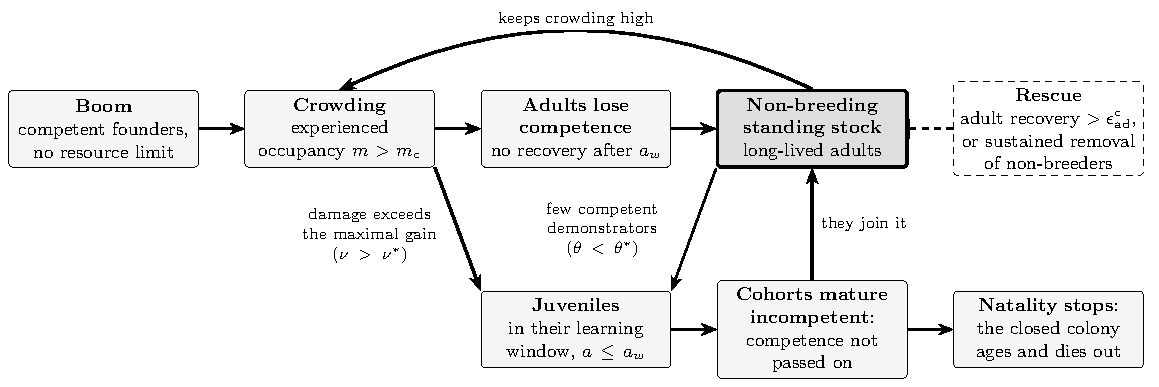
\includegraphics[width=\textwidth]{fig_causal.pdf}
  \caption{Causal scheme of the collapse. Thick arrows form the reinforcing loop. Crowding makes adults lose their
  reproductive competence. After the sensitive window ($a>a_w$) the loss is permanent, and the long-lived
  non-breeders (a standing stock of non-breeding adults) keep crowding high: in space during the
  aggregated growth, in the well-mixed limit by holding the density above $\nu^*$ (sufficiency conjectural;
  Section~\ref{sec:res-mechanism}). Juveniles in their window are then damaged faster than they can learn. They
  also learn from few competent demonstrators ($\theta<\theta^*$, a precursor), so they mature incompetent and join
  the standing stock, and natality stops. Whether adults recover is the condition of the mechanism (dashed): above a
  threshold $\eadult^c$ of adult recovery the colony persists (Fig.~\ref{fig:recovery}); a sustained removal of
  non-breeders also rescues it. Protecting only the juveniles, with perfect demonstrators or a crowding-free
  nursery, does not (798 of 800 colonies went extinct; SM, Section~\ref{SM-supp:recovery}). Every step acts on
  individuals.}
  \label{fig:causal}
\end{figure}

\section{Methods}
\label{sec:methods}

\subsection{Model}
\label{sec:model}

The model description follows the ODD protocol \citep{Grimm2020}; the full ODD and the code are
in the Supplementary Material (SM, Section~\ref{SM-supp:odd}). The model is individual based and stochastic, with
one time step per week. Individuals live in a closed arena of $|G|=L\times L$ cells ($L=30$). A cell stands for a
nest site or local group: it is the unit at which crowding is experienced and mates are met. Each individual has an
age $a$, a sex, a position and a \emph{reproductive competence} $s\in[0,1]$, a phenomenological scalar that summarises
the capacity to breed, the capacity to rear young and the quality of the individual as a demonstrator for juveniles.
There are no resources and no predators, and no individual knows the population size. The simple interaction rules
of the title are all the rules below: the core processes, among them crowding damage and senescence, which suffice
for the collapse (Section~\ref{sec:res-wm}), and four social rules, which add specific patterns.
Table~\ref{tab:params} lists the key parameters.

\paragraph{Core processes}
\emph{Crowding damage.} Each week, after moving, competence is updated with the occupancy $m_i$ of the cell of $i$,
itself included:
\begin{equation}\label{eq:stress}
  s_i\leftarrow\min\{1,\max[0,\;s_i+g_i-\gamma\,(m_i-m_c)_+]\},
\end{equation}
where $g_i$ is the weekly gain (below), $m_c$ the tolerated group size and $\gamma$ the damage per extra occupant. In
Universe~25 social disruption arose while food and water were in excess \citep{Calhoun1973}, so the rule is
interference without a resource. It responds to the crowding that an individual experiences, not to the density
$N/|G|$.
\emph{Competence gates breeding and care.} A reproductive female that shares her cell with a reproductive male
(chosen at random) conceives with probability $p_0s_fs_m$; each pup survives birth with probability $q_0s_f$ and
starts with a fraction $w$ of its mother's competence,
\begin{equation}\label{eq:breed}
  p_{\rm conc}=p_0\,s_f\,s_m,\qquad p_{\rm surv}=q_0\,s_f,\qquad s_{\rm pup}=w\,s_f.
\end{equation}
The last relation is a maternal effect \citep{GinzburgTaneyhill1994}, not inheritance; it is an
assumption of \Cone, not an ingredient of the mechanism ($w=0$ with faster learning gives the same outcome,
Section~\ref{sec:res-patterns}). The rule encodes the failures that Calhoun reported in the crowded phase: males that
ceased courting, and mothers that abandoned their litters.
\emph{Senescence and attraction.} Death is senescent, with weekly hazard $[1+e^{-k(a-a_{\max})}]^{-1}$, independent
of $s$; females breed between $a_{\min}$ and $a_{\rm rep}$ weeks of age. These values follow Universe~25: menopause at
about $560$ days, many mice alive at about $800$ days, and withdrawn animals that were ``physically healthy''
\citep{Calhoun1973}. Each week every individual moves to a cell $y$ of its $3\times3$ neighbourhood (own cell
included) with probability proportional to
\begin{equation}\label{eq:move}
  W_i(y)=\bigl[1+\alpha\,\chi_i(y)\bigr]\;e^{-\kappa(1-s_i)^{p}n_y}\;\bigl[1+\pi(1-s_i)^{q}\,\mathbf 1_{\mathcal R}(y)\bigr],
\end{equation}
where $n_y$ is the number of other individuals in $y$ and $\chi_i(y)$ the summed affinity of $i$ for them; affinities
grow by proximity and decay with a memory of about 100 weeks. The first factor, attraction to acquaintances,
aggregates the colony, in the spirit of Calhoun's ``behavioural sink'' \citep{Calhoun1962}.

\paragraph{Four social rules}
The four social rules are labelled as in the code and in the figures.
\emph{Sensitive window (R1).} Competence can be gained only up to age $a_w$, a window that spans weaning and
maturity ($g_i=0$ for $a_i>a_w$), while crowding damage acts at every age. Mice removed from a declining companion
colony bred very poorly in uncrowded enclosures: after two months without reproduction, half of the females
conceived with normal males and 5 of about 100 pups survived \citep{Marsden1972}. The rule is the standard form of a
developmental sensitive window \citep{FawcettFrankenhuis2015}. Of all the assumptions, adult irreversibility has the
least empirical support and the largest effect; a variant multiplies the adult gain by a factor $\eadult\in[0,1]$,
the adult recovery factor (\Cone: $\eadult=0$).
\emph{Social learning of competence (R2).} Inside the window the gain is set by the neighbours,
\begin{equation}\label{eq:learning}
  g_i=r\bigl[(1-\lambda)+\lambda\,\bar s_{V(i)}\bigr]\qquad(a_i\le a_w),
\end{equation}
where $\bar s_{V(i)}$ is the mean competence of the other individuals of the $3\times3$ block around $i$ (zero if
there are none); \Cone\ has $\lambda=1$, purely social learning. A pup starts at $ws_f\le0.2$ and can gain at most
$ra_w=1.2$, but only among competent demonstrators. The rule follows Calhoun's observation that ``by midway in
phase~C essentially all young were prematurely rejected by their mothers''; it is consistent with the non-genomic
transmission of maternal care in rats \citep{Francis1999} and the social learning of pup retrieval in mice
\citep{Carcea2021}, which support the social transmission of maternal care, not of male sexual competence, which
the model extends by hypothesis.
\emph{Crowd aversion (AV) and retreat sites (R7).} The second factor of Eq.~\eqref{eq:move} makes deteriorated
animals ($s\lesssim0.3$) avoid crowded cells, and the third makes them prefer retreat sites, a fraction $f_R$ of the
cells that hold at most $c_R$ individuals. They follow Calhoun's descriptions of withdrawn males that pooled in the
centre, ``beautiful ones'' that never fought, and withdrawn females that retreated to the high, less-preferred nest
boxes \citep{Calhoun1973}.

\begin{table}[!tp]
\centering
\caption{Key parameters of the reference model \Cone\ (SM, Table~\ref{SM-tab:odd-params}, for all parameters and
their justification). The short-lived control differs in $a_{\max}=60$, $a_{\rm rep}=50$, $r=0.01$, $\lambda=0$,
$a_w=\infty$, $w=1$, $\alpha=1.4$ and has neither crowd aversion nor retreat sites.}
\label{tab:params}
\footnotesize
\setlength{\tabcolsep}{3pt}
\begin{adjustbox}{max width=\textwidth}
\begin{tabular}{@{}llp{4.0cm}llp{4.0cm}@{}}
\toprule
Symbol & Value & Meaning & Symbol & Value & Meaning \\
\midrule
$L$ & 30 & side of the arena ($|G|=900$ cells) & $r$ & 0.1 & maximal weekly gain of competence \\
$N_0$ & 200+200 & founders, age 4 weeks, $s=1$ & $a_w$ & 12 weeks & sensitive window (R1) \\
$m_c$ & 8 & tolerated occupancy & $\lambda$ & 1 & weight of social learning (R2) \\
$\gamma$ & 0.1 & damage per extra occupant & $\eadult$ & 0 & adult recovery factor \\
$p_0$ & 0.3 & weekly conception probability & $w$ & 0.2 & maternal transmission \\
$q_0$ & 0.95 & pup survival at $s_f=1$ & $\alpha$ & 4 & attraction to acquaintances \\
litter & 3--10, mean 6.55 & litter size & $\kappa$, $p$ & 0.15, 4 & crowd aversion (AV) \\
$a_{\min}$, $a_{\rm rep}$ & 6, 80 weeks & reproductive ages of females & $f_R$, $c_R$ & 0.3, 2 & retreat sites (R7) \\
$a_{\max}$, $k$ & 120 weeks, 0.15 & senescence & $\pi$, $q$ & 100, 4 & preference for retreat sites (R7) \\
\bottomrule
\end{tabular}
\end{adjustbox}
\end{table}

\paragraph{Order of processes and demography}
Each week, in this order: every individual moves (Eq.~\ref{eq:move}, simultaneously, with the capacity of the
retreat sites enforced); affinities are updated; occupancies are counted; competence is updated
(Eqs.~\ref{eq:stress} and~\ref{eq:learning}); females mate in their cell, conceive and give birth to the pups that
survive, which are placed in the mother's cell; individuals age and die; observables are recorded. The founders,
$200$ females and $200$ males of age 4 weeks with $s=1$, are placed at random. Four simplifications of mouse
demography have measured effects (SM, Fig.~\ref{SM-fig:robustness}). There is no gestation or interbirth interval:
conception and birth occur in the same weekly step, with a ceiling of about two pups per female and week; with a
refractory period of three weeks after each birth \Cone\ still collapses (60 of 60 runs extinct with either of two seed
sets; joint outcome 59 of 60 with an independent seed and 60 of 60 with the production seeds), and the extinction
time changes by $+1.0$ [$-2.6$, $4.6$] weeks (paired with the production seeds). Pups move
and add to crowding from birth; keeping them in the maternal cell for three weeks lowers the joint outcome (below) to
0.83. The founders form a synchronous cohort, and 69\% of all births are theirs; initial ages spread over 4--80 weeks
give 0.63. There is no mortality before senescence; a background mortality of 0.003 per week lowers the joint
outcome to 0.55 and 0.008 to 0.06, in both cases through the timing of the end of natality, while up to 0.05 per
week does not rescue the colony (SM, Section~\ref{SM-supp:recovery}). Longevity is part of the mechanism, not a detail
(Section~\ref{sec:res-mechanism}).

\paragraph{Model structures compared}
The reference model \Cone\ has the core processes and the four social rules. The \emph{core model} keeps the core
processes but replaces the four social rules by neutral values: no window, individual recovery at a slow rate ($r=0.01$) at every age,
full maternal transmission ($w=1$), no crowd aversion and no retreat sites. A null model has no crowding damage
($\gamma=0$). The \emph{short-lived control} (Table~\ref{tab:params}) regenerates competence individually; in space 89
of its 200 colonies are still alive at week $1\,000$, cycling with a period of 162 [155, 170] weeks. The
\emph{reversible-suppression null} is \Cone\ with the two recovery parameters changed: adults recover at a fraction
$\eadult=0.8$ of the juvenile rate, and $\lambda=0.9$ instead of 1 keeps social learning but lets them recover partly
on their own, at the asocial rate $\eadult(1-\lambda)=0.08$ of the juvenile rate. With $\lambda=1$, $\eadult=0.8$
lies inside the transition (10 of 20 colonies die out at $L=30$); the null lies above the rescue threshold at every
size simulated (Section~\ref{sec:res-recovery}). The parameters that set the form of the rules were chosen to reproduce the most
qualitative patterns with the fewest rules; they were not fitted to Calhoun's curves. In the \emph{well-mixed}
variants every individual moves each week to a uniformly random cell, so that attraction, aversion and the
preference for retreat sites have no effect and the retreat sites act only as a capacity; cell occupancies are
Poisson with mean $N/|G|$. A female then mates either within her cell, as in space (\emph{local mating}), or with a
reproductive male drawn from the whole arena (\emph{global mating}), which removes any difficulty of finding a mate.

\subsection{Patterns, evaluation and statistical design}
\label{sec:patterns}

From Calhoun's report we extracted seventeen qualitative, falsifiable patterns and four anti-patterns, each
translated into an operational criterion on simulated time series (SM, Table~\ref{SM-tab:observations-full}; codes
in parentheses). Growth: latency, exponential growth and deceleration (O1--O3, scored only with a separate founder
protocol from four pairs), and a socially functional growth phase (O10b). Peak: a peak far below capacity with empty
nest sites (O4), adults that deteriorate before it (O10), aggregation with free space (O14), and coexisting crowded
and withdrawn non-breeders (O13), with a persistent withdrawn class (O13p) born late (O13b). Decline: late-born
cohorts that fail to mature (O11) and rarely conceive (O11b), natality that ceases near the peak (O5), no recovery of
natality (O6), extinction (O7), a long senescent decline (O8) to an old, female-biased remnant (O9), total infant
mortality (O15), and the failure of transplanted late animals to breed (O12). We call O5, O6, O7 and O10 the
\emph{collapse envelope}. Calhoun's dates enter only through dimensionless ratios of the time and size of the peak.
A criterion returns PASS, MARGINAL (one step from its threshold), FAIL or not applicable for each run, and an
ensemble is summarised by the fraction of passing runs with a 95\% Wilson score interval. The joint
outcome O17p requires every applicable essential pattern, no anti-pattern and a persistent withdrawn class. Every run
was scored with the evaluator preregistered before the production runs (a time-stamped plan in the code repository,
1 October 2026; SM, Section~\ref{SM-supp:evaluators}) and with a primary evaluator, fixed before those runs, that dates the peak at the start of the plateau rather than at $\arg\max N$; the two are reported side
by side (SM, Table~\ref{SM-tab:res-rescoring}). One option, the end of natality in O5 at the week by which 99\% of the
births have occurred, was chosen after exploratory runs had shown that the last sustained birth fails O5 in about
half of the \Cone\ runs (with that reference O17p is 0.485, 97 of 200 production runs). Square brackets give 95\% intervals unless
stated otherwise.

The unit of analysis is the independent stochastic replicate. The design comprises production ensembles of the model
structures ($n=200$ each), a factorial ablation of the rules, transplant experiments ($60$ replicates per arm), a
sweep of the adult recovery factor at three arena sizes, robustness variants, lattice sizes, and a global
sensitivity analysis (Morris screening, two Latin hypercubes and Sobol' indices); seven
confirmatory hypotheses were tested with Holm correction, and extinction times are summarised by Kaplan--Meier
estimates (SM, Sections~\ref{SM-supp:Q} and~\ref{SM-supp:ensembles}).

\paragraph{Use of AI in the research}
Starting from the author's preliminary implementation and draft rules, Claude (Anthropic) agents, used through Claude
Code (v2.1; Claude Opus 5.5 and Claude Fable 5.1 for the research tasks, Claude Sonnet 5.5 for literature searches and
auxiliary programming), reimplemented and extended the code, ran the simulations and the statistical analyses, and
searched the literature. The author set the objectives, the qualitative targets and the interaction rules, decided
every change of scope and approved each stage. The code has an automated test suite; scripts in the code repository
regenerate every figure and number from the archived outputs; independent Claude agents reviewed the work, checking
the code against the text and reproducing key results; and the history is kept under version control.

% Results. Numbers: results_em/ (see README.md of the repository).
\section{Results}
\label{sec:results}

\subsection{The reference colony follows Calhoun's sequence}
\label{sec:res-trajectory}

The time course of \Cone\ has the four phases of Universe~25 in Calhoun's order (Fig.~\ref{fig:trajectory}). On a
time axis relative to the peak of each system ($t_{\rm pk}$: the start of the plateau in the model, median week 34;
day 560 in Universe~25), births start at $0.09\,t_{\rm pk}$ and growth slows at $0.31\,t_{\rm pk}$ (Universe~25: 0.19
and 0.56). The mean competence of the adults falls below 0.5 at week 13, while the colony is still growing. Births
stop near the peak: 99\% of them have occurred by week 40 and the last one comes at week 59 [46, 76] (median and
10--90\% range over 200 runs). The shapes differ after the peak. The model stays on a plateau for about
$1.5\,t_{\rm pk}$ and then falls along a sigmoid as the closed cohort ages, whereas Universe~25 declined from its
peak; the model dies out at $4.97\,t_{\rm pk}$, week 169 (Kaplan--Meier median; 95\% interval [167, 171]; 10--90\%
range [157, 186]), against a projected $3.18\,t_{\rm pk}$ for Universe~25. The peak uses $0.36$ of the
damage-threshold capacity $\Kg=m_c|G|$ and leaves 16\% of the cells empty (Universe~25: about 20\% of the nest boxes
empty, an agreement in sign, since $|G|$ and $m_c$ were not calibrated). The model starts from 400 young adults
rather than four pairs, so the comparison is of shape, not of timing (doubling times: SM,
Section~\ref{SM-supp:patterns}).

\begin{figure}[!tp]
  \centering
  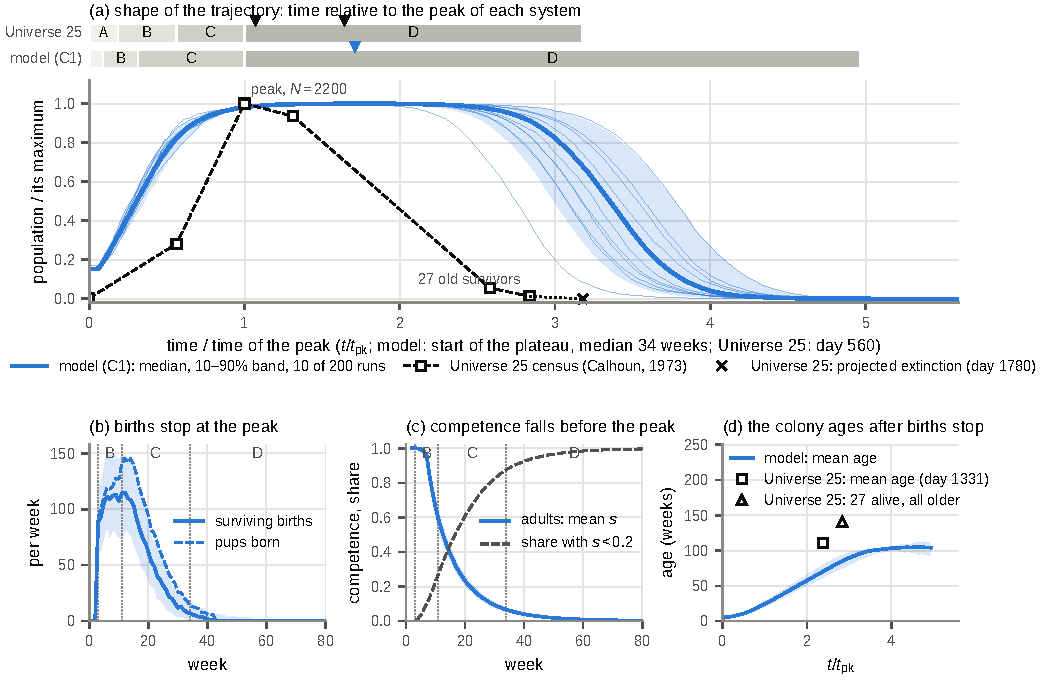
\includegraphics[width=0.9\textwidth]{fig_em_trajectory.pdf}
  \caption{The reference colony and Universe~25. (a)~Population relative to its maximum against time relative to
  the peak of each system, $t/t_{\rm pk}$ ($t_{\rm pk}$: start of the plateau, $N\ge0.98\max N$, in each run of the
  model, median week 34; day 560 in Universe~25). Model: \Cone, median, 10--90\% band and 10 of 200 colonies,
  rescaled run by run. Squares: census of Universe~25 \citep{Calhoun1973}; cross: Calhoun's projected extinction
  (day $1\,780$). Ribbons: phases A--D (A, adjustment; B, growth; C, slower growth; D, death phase) as dated by
  Calhoun and, for the model, as measured in each run (medians): first births, halving of the growth rate of $\ln N$,
  start of the plateau and extinction. Triangles: last surviving young and last conception in Universe~25, last birth
  in the model. No curve is fitted. (b)~Pups born and pups surviving birth per week. (c)~Mean reproductive
  competence of the adults and share of all animals with $s<0.2$. (d)~Mean age of the living animals against
  $t/t_{\rm pk}$; symbols: mean age of the survivors of Universe~25 on day $1\,331$, and the 27 survivors on day
  $1\,588$, all older than 987 days. Bands: 10--90\% of colonies. Dotted lines in (b, c): phase boundaries.}
  \label{fig:trajectory}
\end{figure}

\subsection{Adult recovery decides the outcome}
\label{sec:res-recovery}

Whether adults made non-breeding by crowding recover decides between collapse and persistence
(Fig.~\ref{fig:recovery}). If adults regain competence at a fraction $\eadult$ of the juvenile rate, every colony
still dies out for $\eadult\le0.02$ ($2\,880$ of $2\,880$ colonies at $L=15$ and 30, in space and well mixed, for
every $\lambda$; SM, Table~\ref{SM-tab:sm-pext}), so the collapse is not an artefact of the edge $\eadult=0$. Above a
threshold $\eadult^c$ the colony persists. In space the threshold falls with the side of the arena without visible
saturation: from 0.133 [0.113, 0.157] to 0.085 [0.073, 0.099] and 0.050 [0.037, 0.063] between $L=15$, 30 and 60
when recovery is individual ($\lambda=0$), and from 0.97 [0.88, $>$1] to 0.73 [0.67, 0.81] and 0.53 [0.46, 0.62]
when it is purely social ($\lambda=1$; profile-likelihood intervals of the midpoint; SM, Table~\ref{SM-tab:sm-epsc}).
Three sizes do not determine its limit for $L\to\infty$, which could be zero. Well mixed with global mating it also
falls (0.81, 0.51, 0.30, again with non-overlapping intervals); with mating in the cell it is resolved only to the
grid of $\eadult$ (0.80, 0.6--0.8, 0.60; overlapping intervals), compatible with the deterministic limit, 0.585.
With $\lambda\ge0.9$ no recovery rescues the well-mixed colony (all but one of $4\,860$ colonies die out), because
an adult whose recovery is social finds no competent demonstrators. The robust statement is therefore the edge: the collapse requires that adults recover
asocially at most slowly, $\eadult(1-\lambda)\approx0$, at the scale of the experiment.

The reversible-suppression null, \Cone\ with $\eadult=0.8$ and $\lambda=0.9$ (asocial recovery at 0.08 of the
juvenile rate), persists in all 200 colonies to week
$1\,000$. It keeps every spatial and deterioration pattern of \Cone\ (200 of 200 runs each; Fig.~\ref{fig:patterns},
first 600 weeks), and its natality nearly ceases after the peak (to 0.1\% of its maximum, median), so the two
outcomes share the first half of the sequence; but breeding then resumes. The collapse envelope separates them: the
end of natality, the absence of recovery and the extinction fail in all 200 runs. Nor does the colony settle. After
a plateau from week 34 to about week 100 (median) it falls to 0.15 of the peak (week 141) and then cycles with a
period of 148 [147, 149] weeks (peak to peak; mean over runs, 143--152 across runs, 10--90\%). The oscillations are
persistent and slowly damped. The peak-to-trough amplitude decays from 0.85 of the first peak to 0.49, 0.42 and 0.39
in the next three cycles and then only slowly ($-0.013$ [$-0.017$, $-0.008$] of the first peak per 100 weeks over
cycles 3--5, about 3\% of the amplitude), so that at week $1\,000$ the colony still oscillates between about 0.40
and 0.80 of the first peak. Whether the amplitude levels off (a geometric fit gives 0.35 [0.33, 0.37]) or keeps
decaying cannot be decided within $1\,000$ weeks. The autocorrelation of $N$ over weeks 300--1000, corrected for the
shrinking overlap of the lagged series, is 0.90 at one, two and three periods (0.71, 0.51 and 0.34 uncorrected),
which rules out a fast-relaxing quasi-cycle. In all 200 runs the evaluation
thus finds cycles with recovery of births and no logistic saturation: the trajectory differs in form, not only in
level. With initial ages spread over 4--80 weeks the null falls to 0.23 [0.21, 0.25] of the peak and cycles with the
same period, so the cycle is not an artefact of the synchronous founding cohort.

Earlier confined colonies, not used to build or tune the model, allow only a consistency check of this branch,
since its persistence follows from the choice of $\eadult$ above the threshold. With food in excess those colonies
stopped growing below the limit set by food, mainly through the failure of litters to survive
\citep{Southwick1955a,Southwick1955}; confined populations of several rodent species regulated their density
\citep{Lidicker1965}; and confined deermice of asymptotic populations did not breed until removed from them
\citep{Terman1973}. Scored on the null (re-run with the archived seeds to record every litter), litter loss is
concentrated on the plateau: the fraction of litters with no surviving pup rises from 0.05 during growth to 0.24
[0.24, 0.25] (0.09 in \Cone) and falls back to 0.07--0.10 afterwards. But the fall of natality is mainly a fall of
conception (73\% of its logarithmic decline), so this pattern is reproduced only in part. Most females born on the
plateau never breed (0.89 do not conceive by 48 weeks of age), but so do those of \Cone\ (0.96). In \Cone\ no female
is born after the plateau, whereas in the null those born during the decline breed (only 0.37 do not conceive by 48
weeks; 0.72 of those born from week 300 on); what separates the outcomes is whether adults resume breeding
(definitions and sources of these held-out patterns: SM, Section~\ref{SM-supp:recovery}). The quick recovery of deermice removed from the asymptotic population
is reproduced by construction: phase-D animals of \Cone\ moved to an enclosure where adults recover
individually found a colony in 51 of 60 trials (Fig.~\ref{fig:behaviour}e), whereas Calhoun's transplants bred very
poorly \citep{Marsden1972}, the pattern of the irreversible branch.

\begin{figure}[!tp]
  \centering
  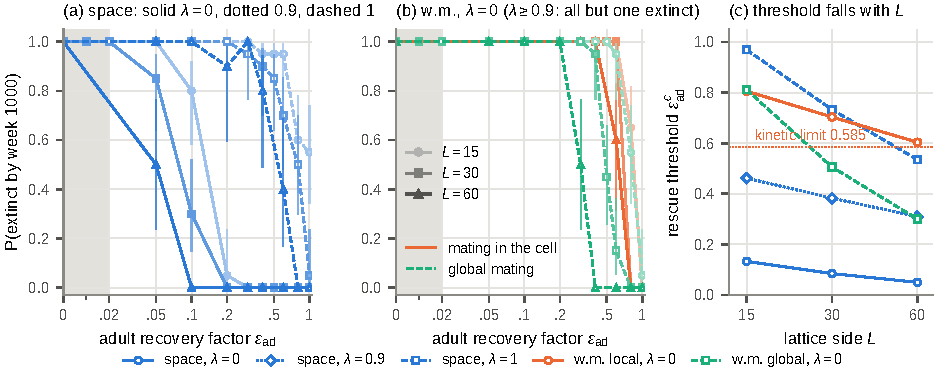
\includegraphics[width=\textwidth]{fig_em_recovery.pdf}
  \caption{Adult recovery decides the outcome. Probability that a \Cone\ colony is extinct by week $1\,000$ against
  the adult recovery factor $\eadult$ (fraction of the juvenile rate). (a)~Spatial model (with retreat sites),
  individual ($\lambda=0$, solid), mostly social ($\lambda=0.9$, dotted) or purely social recovery ($\lambda=1$,
  dashed). (b)~Well-mixed model, $\lambda=0$, mating in the cell (orange) or global (green); with $\lambda\ge0.9$ all
  but one of the $4\,860$ well-mixed colonies (three mating rules) die out. Shades and markers: $L=15$, 30, 60 (20, 20 and 10 colonies per point; 95\% Wilson intervals
  where $0<P<1$). Grey band: every colony collapses. (c)~Rescue threshold $\eadult^c$ (midpoint of a logistic fit)
  against $L$; dotted: value of the kinetic equation, 0.585. Data: SM, Tables~\ref{SM-tab:sm-pext}
  and~\ref{SM-tab:sm-epsc}.}
  \label{fig:recovery}
\end{figure}

\subsection{The collapse needs neither space nor the four social rules}
\label{sec:res-wm}

Removing space requires a control (Fig.~\ref{fig:wellmixed}e). When every animal is relocated at random each week
but mates only within its cell, the deformation is extinctive in itself: the short-lived control, which in space is
still alive in 89 of 200 colonies at week $1\,000$, dies out in 200 of 200 well-mixed colonies (median 120 weeks,
earlier than \Cone, 147), through a mate-finding Allee effect after the overshoot. The test therefore rests on
global mating, in which a female mates with a reproductive male drawn from the whole arena. There the control lives
far longer than \Cone\ and persists in larger arenas (extinct by week $1\,000$: 81, 1 and 0 of 200 at $L=30$, 45
and 60; at $L=30$ all colonies die out by week $3\,000$), whereas \Cone\ dies out in all 600 colonies at 138--140
weeks, almost independently of $L$. The core model without the four social rules collapses as well, in space and in
both well-mixed variants (all $1\,000$ colonies; median extinction at 136--166 weeks). The core model and the
short-lived control share the same slow individual recovery at every age ($r=0.01$); well mixed, where attraction
($\alpha$, 4 in the core and 1.4 in the control) plays no role, only the long life span of the core makes it
collapse. The cessation of breeding and the extinction thus need neither space nor the four social
rules: they need crowding damage and long-lived adults that recover slowly, if at all
(Section~\ref{sec:res-recovery}). A component
Allee effect remains with global mating, because a female paired with an incompetent male conceives with
probability $p_0s_fs_m$.

Without space the end of natality and the extinction are the same, but the sequence is not. With mating in the
cell, growth stays fast and competent until the peak (a socially functional growth phase in 200 of 200 runs, against
4 of 200, and 194 marginal, in space), the peak is 2.3 times denser (6.6 against 2.9 animals per cell), and
competence then collapses at once, so that phase~C lasts two weeks (weeks 24--26), against 23 weeks in space and
about 35 in Universe~25. With global mating phase~C lasts 11 weeks (weeks 7--18), so the compression comes from local
mating, not from the absence of space. Space also changes how the colony is organised. At the spatial
peak the mean occupancy is 2.9 animals per cell, but it is aggregated (variance-to-mean ratio 2.53 [2.51, 2.55];
maximum about 16) and 18\% [18, 19] of the animals sit in cells above $m_c$ (SM, Figs.~\ref{SM-fig:occupancy}
and~\ref{SM-fig:snapshots}): the colony crowds into pools next to empty cells and lodges a class of withdrawn
non-breeders, isolated adults with $s<0.2$ that appear already during growth and sit mostly in the retreat
sites; well mixed the occupancy is homogeneous and almost nobody stays isolated. That class cannot form under random
relocation, so its absence there is a consistency check, not a finding.

\begin{figure}[!tp]
  \centering
  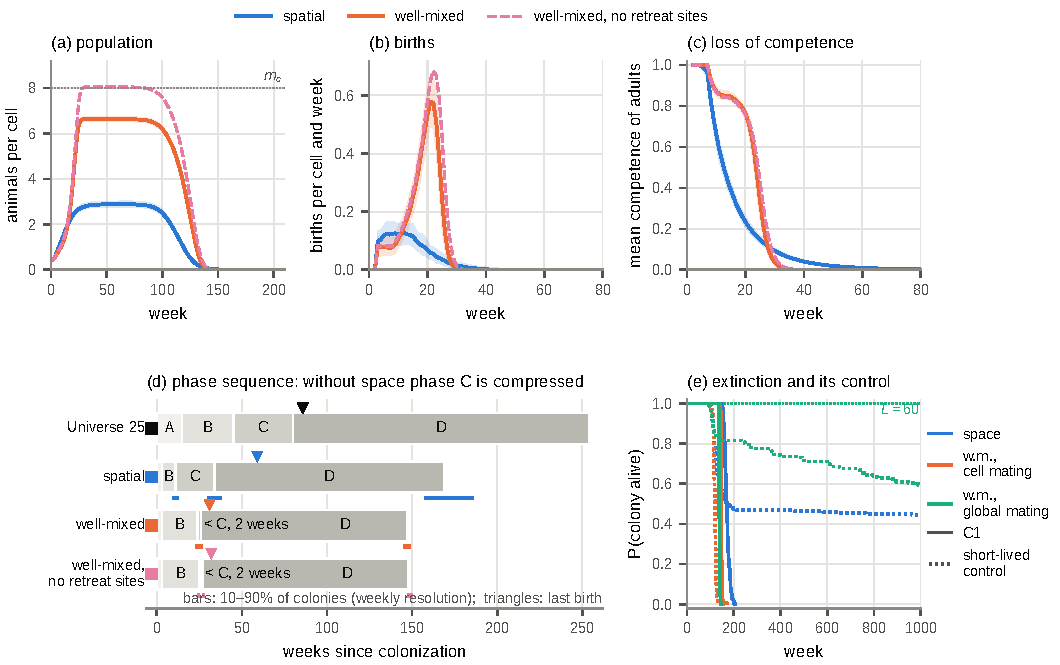
\includegraphics[width=0.92\textwidth]{fig_em_wellmixed.pdf}
  \caption{Extinction with and without space, and its control. Spatial \Cone\ (blue, $n=200$) and well-mixed \Cone,
  in which every animal is relocated at random every week and mates in its cell (orange, $n=200$; retreat sites act
  only as a capacity; pink dashed, without retreat sites, $n=200$); $L=30$, 400 initial animals. (a)~Animals per
  cell; dotted line: the tolerated crowding $m_c$. (b)~Births per cell and week. (c)~Mean reproductive competence of
  the adults. Medians with 10--90\% bands. (d)~Phase sequence of Universe~25 and of each model, dated as in
  Fig.~\ref{fig:trajectory} (medians; bars below: 10--90\% of the colonies at weekly resolution; triangles: last
  birth). With mating in the cell phase~C lasts two weeks. (e)~Kaplan--Meier survival to week $1\,000$ of \Cone\
  (solid) and of the short-lived control (dotted) in space, well mixed with mating in the cell, and well mixed with
  global mating ($L=30$; the control with global mating also at $L=60$, where no colony dies out). Global mating
  appears only in panel~(e). Maps of one colony at its peak and in its decline: SM, Fig.~\ref{SM-fig:snapshots};
  full sequences: Supplementary Videos S1--S3.}
  \label{fig:wellmixed}
\end{figure}

\subsection{Which rule produces which pattern}
\label{sec:res-patterns}

The pattern matrix filters structures through the collapse envelope (Fig.~\ref{fig:patterns}). The envelope passes
in every column with crowding damage and long-lived adults that do not recover fast, except that adult deterioration
before the peak is only partial in the well-mixed core (0.78 of runs with mating in the cell and 0.18 with global
mating): with global mating the core reproduces the end of natality and the extinction, but not
the deterioration of adults before the peak. The envelope fails in the two reversible structures, the
reversible-suppression null and the short-lived control. Without crowding damage the colony explodes (every run
reaches the numerical cap of $15\,000$ animals at weeks 26--29, median 27). The spatial patterns, a peak far below capacity with empty nest sites and
aggregation with free space, pass in every spatial column with crowding damage and in no well-mixed one. All
essential patterns jointly hold in 0.995 [0.97, 1.00] of the runs of \Cone\ (199 of 200) and in none of the other
columns. The senescent nature of the decline holds by construction (there is no social mortality), but its duration
criterion passes in 0.62 of the \Cone\ runs; the persistence of the withdrawn class follows from the capacity of the
retreat sites, which equals the isolation threshold; the failure of transplanted adults follows from R1; and in the
well-mixed columns the coexistence of crowded and withdrawn non-breeders is arithmetic, not behaviour
(Fig.~\ref{fig:patterns}).

The ablations name the rule behind each pattern (SM, Fig.~\ref{SM-fig:ablations}). Without the sensitive window (R1,
adults recovering socially) the envelope is lost (extinction in 0.23 of the runs); without social learning (R2) only
the failure of the late cohorts; without retreat sites (R7) only the persistence of the withdrawn class; without crowd
aversion only the timing clause of the end of natality (0.82) and the duration of the decline. The core model keeps
the envelope in space and loses the cohort failure, the coexistence of classes and their persistence. Over two Latin
hypercubes of 15 factors, 353 of 400 parameter points (0.88, 95\% interval 0.85--0.91) reproduce the collapse
envelope, 168 add the failure of the late cohorts, and 9 reproduce every essential pattern (0.022). The collapse is
generic once adults do not recover; what is rare is its conjunction with the spatial and class patterns. Maternal
transmission is not needed ($w=0$ with faster learning gives 1.00), and at fixed seeding density the joint outcome
rises from 0.82 at $L=15$ to 1.00 at $L\ge45$ (SM, Fig.~\ref{SM-fig:robustness}).

Of the seven confirmatory predictions fixed before the production runs, three fail with each evaluator (SM,
Section~\ref{SM-supp:Q}). Q2, that each rule is necessary, fails because without crowd aversion the joint outcome
stays at 0.79 [0.71, 0.86] (0.90 with the preregistered evaluator) against the predicted $\le0.5$; Q5, a band of
coexisting crowded and withdrawn non-breeders centred at the preferred occupancy, is refuted in the opposite
direction; and Q6, that the window weighs less than the learning rate, fails with the primary evaluator and holds
with the preregistered one. Q1, the failure of transplanted late animals, holds with the primary evaluator but not
with the preregistered one, which takes the transplants at $1.75$ times the week of $\arg\max N$, later in the
plateau: 12 of 60 groups found a colony ($P_T=0.20$ [0.12, 0.32]). Q3, Q4 and Q7 hold with both.

\begin{figure}[!tp]
  \centering
  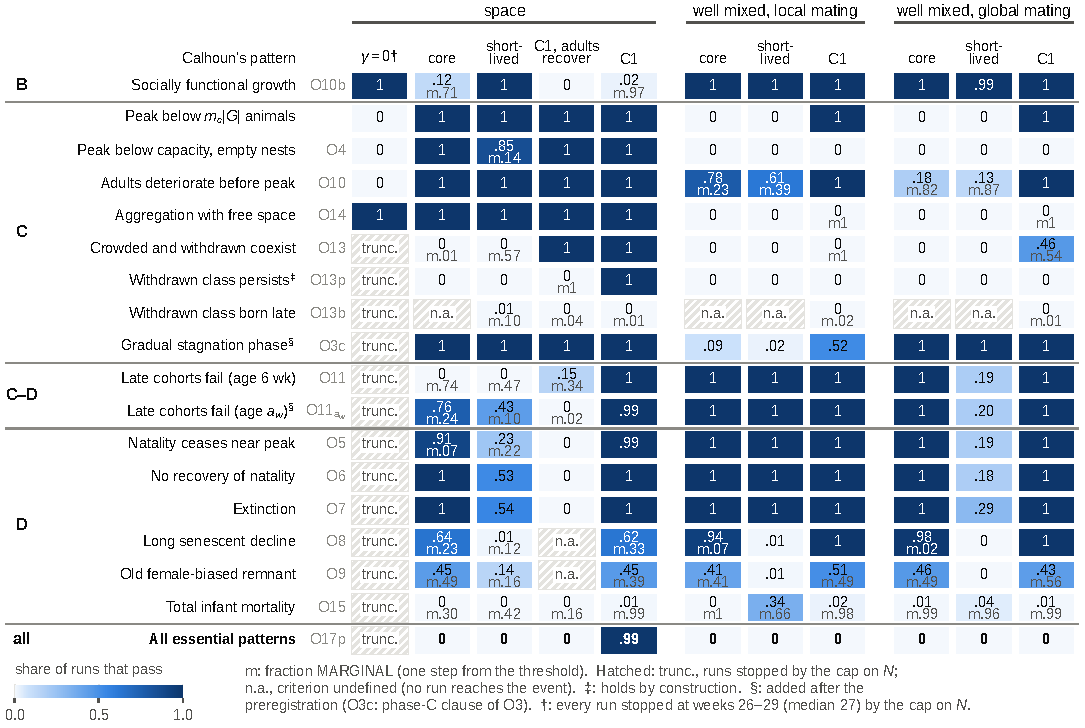
\includegraphics[width=\textwidth]{fig_em_patterns.pdf}
  \caption{Which model structures reproduce Calhoun's patterns. Colour and upper number: fraction of runs that pass
  the operational criterion (primary evaluator, $n=200$ per column, $L=30$, $T=600$; Wilson half-width $\le0.07$);
  lower number (m): fraction MARGINAL, one step from the threshold. Columns: in space, no crowding damage ($\gamma=0$;
  $\dagger$every run stops at weeks 26--29, median 27, when $N$ reaches the numerical cap of $15\,000$, so only
  criteria decided before the cap are shown), the core model (crowding damage, maternal transmission, senescence and attraction,
  without R1, R2, AV and R7), the short-lived control, \Cone\ with adults that recover ($\eadult=0.8$,
  $\lambda=0.9$) and \Cone; well mixed with mating in the cell, and with global mating, for the core model, the
  control and \Cone. Each column comes from one ensemble and seed set (SM, Table~\ref{SM-tab:res-ensembles}). The
  first row is empirical (peak below $m_c|G|$). In the well-mixed columns the
  coexistence of crowded and withdrawn non-breeders is fixed by the capacity of the retreat sites, and the joint
  outcome is 0 by construction (a withdrawn class cannot persist under random relocation). $\ddagger$: holds by
  construction. $\S$: added after the preregistration (the phase-C clause of O3, $t_D-t_{BC}\ge0.1\,t_D$; O11 at
  age $a_w$).}
  \label{fig:patterns}
\end{figure}

\subsection{Behavioural patterns}
\label{sec:res-behaviour}

The individual-level patterns of Calhoun's report appear in the model, each with its ingredient
(Fig.~\ref{fig:behaviour}). In space, crowded and withdrawn non-breeders coexist and the withdrawn class persists: at
week 60, 18\% of the adults are crowded non-breeders, 28\% withdrawn and 17\% persistently withdrawn; well mixed,
isolation is brief and random (57\%, 9\% and 0.2\%). Maternal care fails with the competence of the mothers: the
share of pups that survive birth falls through the growth phase in both variants. The late-born cohorts never breed:
35\% of the females of the first spatial cohort ever conceive, 11\% of those born in week 13 and 6\% of those born in
week 20 (in a two-cell universe run in parallel with Universe~25, 18\% of 148 females born in the last 50 days of
phase~C had ever conceived by a median age of 334 days; \citealp[p.~85]{Calhoun1973}). The transplants of
\citet{Marsden1972}, whose animals bred very poorly rather than not at all, are reproduced qualitatively: groups
taken in the growth phase found a colony in 52 of 60 trials, and those taken in the death phase in none, alone or
with healthy partners (0/60 and 0/120), by the irreversibility built into R1 (Section~\ref{sec:res-recovery}).

\begin{figure}[!tp]
  \centering
  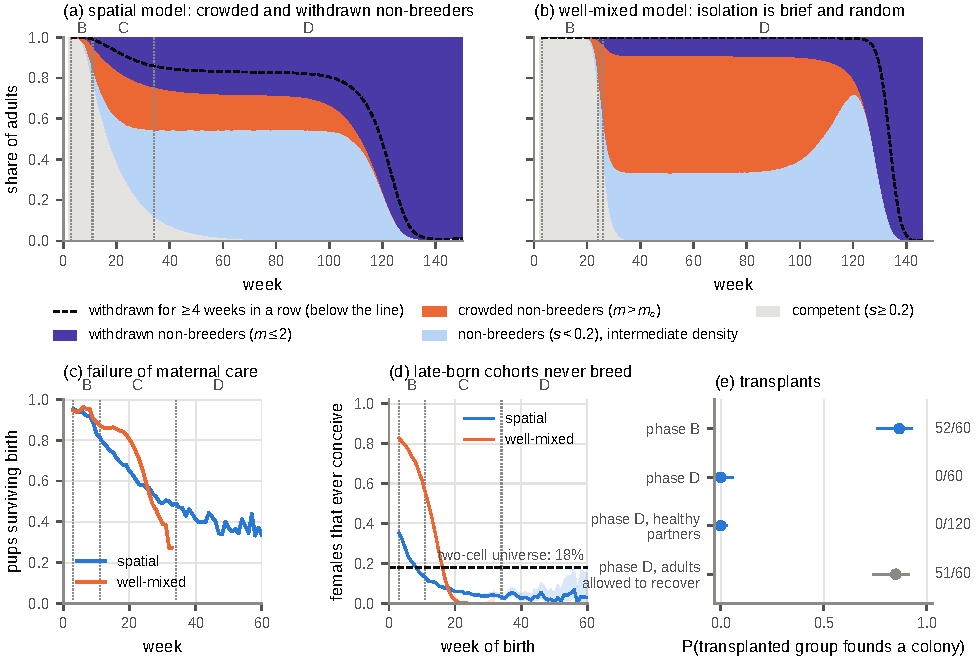
\includegraphics[width=0.9\textwidth]{fig_em_behaviour.pdf}
  \caption{Behavioural patterns. (a,~b)~Composition of the adults (mean over living colonies) in the spatial and the
  well-mixed \Cone: competent ($s\ge0.2$), and non-breeders ($s<0.2$) that are crowded ($m>m_c$), withdrawn (at most
  two animals in the cell) or at intermediate density; below the dashed line, adults withdrawn for at least four
  consecutive weeks. (c)~Share of pups that survive birth, which falls with the competence of the mother (births per
  conception divided by the mean litter size). (d)~Share of the females born in each week that ever conceive, with
  95\% Wilson bands (well mixed: 83\%, 43\% and 2\% for the cohorts born in weeks 3, 13 and 20); dashed line: 18\% of
  the late phase-C females of Calhoun's two-cell universe had ever conceived, a comparison of order (different colony
  and definition). (e)~Transplants (60 groups of four males and four females per arm, 95\% Wilson intervals): a group
  founds a colony when it reaches 80 animals within 150 weeks in an empty enclosure; phase-D animals are taken at
  $1.75\,t'_{\rm pk}$ (primary evaluator). Phase-D animals moved to an
  enclosure where adults may recover (no R1 and R2, individual recovery at rate 0.1) found a colony in 51 of 60
  trials. Dotted lines: phase boundaries of the spatial model (Fig.~\ref{fig:trajectory}).}
  \label{fig:behaviour}
\end{figure}

\subsection{The mechanism}
\label{sec:res-mechanism}

The collapse has the same logic in both structures, a non-breeding state that crowding induces and that adults
cannot leave, but the step that drives it differs. In space, aggregation crowds the adults during growth: the
crowding experienced by juveniles, $\gamma\,\mathrm{E}(m-m_c)_+$, exceeds the maximal gain $r$ only during the growth
phase, when the adults lose their competence within weeks; with $\eadult=0$ they never regain it, and the cohorts
that follow have neither the uncrowded window nor competent neighbours. In the well-mixed limit, the long-lived
non-breeders form a standing stock that keeps the mean crowding above a threshold $\nu^*=6.92$, at which the
expected damage to a juvenile equals $r$; in the kinetic equation, the limit of the well-mixed model at fixed
density, the first cohorts fail through damage inside the window before demonstrators become scarce (SM,
Section~\ref{SM-supp:recovery}). A second threshold, the proportion $\theta^*=(1-w)/(ra_w)=2/3$ of neighbours with
$s>0$, a threshold for the transmission of competence between generations, is only a precursor: in the
simulations the mean proportion around juveniles crosses it before natality falls below 5\% of its maximum, by a
median of 15 weeks in space and 3 well mixed, also in colonies that later persist. Which of these statements are
definitions, analytical arguments, conjectures or simulation results is listed in SM Section~\ref{SM-supp:recovery}. Once the
cohorts mature incompetent, natality stops and the closed colony dies out after the residual life span of the last
cohort, 111 weeks after the last birth in space (median) and about 117 well mixed. In the well-mixed limit two
independent conditions make the non-breeding state absorbing: no adult recovery ($\eadult=0$) or purely social
learning ($\lambda=1$), since an adult whose gain is social cannot recover among non-breeders. Nor is the collapse a
mate-finding Allee effect \citep{Gascoigne2009}: well mixed, \Cone\ collapses with mating in the cell, in the
$3\times3$ block or over the whole arena (50 of 50 colonies under each at $L=15$--60; 95\% interval $[0.93,1]$),
whereas the short-lived control persists with global mating for $L\ge45$ (SM, Table~\ref{SM-tab:sm-mate}).

\section{Discussion}
\label{sec:discussion}

\subsection{Collapse and persistence from the same rules}

Simple local rules, none of which knows the size of the population, qualitatively reproduce much of what Calhoun
observed in Universe~25 when adults made non-breeding by crowding do not recover; when adults recover on their own
above a threshold rate, the colony resumes breeding and persists, oscillating rather than levelling off. The
pattern-oriented comparison of structures assigns the ingredients. The collapse needs crowding damage and long-lived
adults that do not recover; it survives every
change of structure that we applied, including the removal of the four social rules and of space, except adult recovery and
a short life span. The four social rules and space add specific patterns: the failure of the
late-born cohorts (social learning in a window), a persistent withdrawn class (retreat sites), the timing of the end
of natality (crowd aversion), and empty nest sites at a low peak with a prolonged stagnation (aggregation).

The mechanism connects old ideas of small-mammal ecology. Social stress from crowding depresses reproduction
\citep{Christian1950}, and an individual state carried across a delay makes density dependence
delayed \citep{GinzburgTaneyhill1994}. The model adds a developmental window in which
competence is learned socially \citep{FawcettFrankenhuis2015,Carcea2021} and shows that, with a long life span and a
non-breeding state that adults cannot leave, these close a loop: the adults whose competence crowding has removed
keep the crowding that prevents the next cohort from acquiring it. The loop acts on a specific class, the long-lived
non-breeders, which explains why indiscriminate mortality does not rescue the colony while their sustained removal
does (SM, Section~\ref{SM-supp:recovery}). The social component of the model is co-presence and
the transmission of a state, not social roles: dominance, male territoriality and reproductive skew, central to
Calhoun's account and to the social organisation of confined wild mice \citep{CrowcroftRowe1963}, are not modelled.

\subsection{Conditions of the mechanism}
\label{sec:conditions}

\paragraph{Irreversibility}
Density-dependent suppression of breeding in rodents is usually considered reversible. In house mice, urine of grouped females
delays puberty in young females \citep{Drickamer1977}, an effect that fades within ten days of ungrouping
\citep{CoppolaVandenbergh1985}. These signals act on the puberty of juvenile
females, the analogue of the juvenile window of the model, which is already reversible; direct evidence on the
recovery of adults that have stopped breeding is limited to deermice \citep{Terman1973}. With adult recovery
switched on, the same rules keep the colony alive, oscillating, instead of collapsing it
(Section~\ref{sec:res-recovery}). Near-irreversibility is
supported only by the transplants from Calhoun's colonies \citep{Marsden1972}, whose animals were several hundred
days old, when reproductive senescence of BALB/c females is already relevant; in \Cone\ the failure of the
transplants is reproduced by construction, not as independent evidence. The conclusion is therefore conditional:
simple rules give the collapse of Universe~25 if adults made non-breeding by crowding do not recover on their own
and live long (well mixed with purely social recovery no colony is rescued even at the juvenile rate, because no
competent demonstrators are left), and a persisting colony if they do recover. The threshold of adult recovery
is the quantity that an experiment on reversibility should estimate.

\paragraph{Scale}
Universe~25 was a single colony of one size. At fixed seeding density the model reproduces the patterns more often
in larger arenas, but the adult recovery that the collapse tolerates in space decreases with the arena, with no sign
of saturation between $L=15$ and 60 (Fig.~\ref{fig:recovery}c). Three sizes do not determine the limit of this
threshold for an infinite arena, which may be zero, so for any adult recovery above zero the spatial collapse may be
a finite-size effect; only the irreversible case is supported at every size simulated. Extinction itself is certain
for any closed colony with crowding damage, because crowding caps the number of animals that can breed and there is no
immigration; what distinguishes collapse from persistence is that the extinction time
of \Cone\ grows only logarithmically with the size of the colony (SM, Section~\ref{SM-supp:recovery}). The mechanism
is thus established at the scale of the experiment; a much larger closed colony would need an even less reversible
non-breeding state.

\paragraph{Timing}
The conjunction of all patterns is sensitive to when natality ends: with a background mortality of 0.003 per week, or
with initial ages spread over 4--80 weeks, it holds in 0.55 and 0.63 of the runs, only through the timing clause of
the end-of-natality criterion. The collapse itself is not sensitive: background mortality up to 0.05 per week does
not rescue \Cone\ (SM, Section~\ref{SM-supp:recovery}), a gestation-like refractory period of three weeks leaves it unchanged
(60 of 60 runs extinct; Section~\ref{sec:model}), and with spread initial ages the reversible null still falls to
0.23 of its peak and cycles (Section~\ref{sec:res-recovery}).

\subsection{Limits of the spatial layer}
\label{sec:spatial-limits}

The spatial patterns are obtained in a regime of mobility opposite to that of Universe~25. The ratio of the mixing
time to the deterioration time, a Damk\"ohler number, is about $1.7\times10^2$ in \Cone\ and at most $4\times10^{-3}$
in Universe~25, where mice crossed the enclosure daily (SM, Section~\ref{SM-supp:odd}): crossing the lattice by
diffusion takes about $1.7\times10^3$ weeks. In Universe~25 the classes arose among mobile animals through behaviour
(male territories, possession of nest boxes, aggression); in the model they arise from aggregation under low
mobility. The size of the withdrawn class is moreover set by a parameter: from week 30 the 270 retreat sites, with
540 places, are about 94\% occupied, so the class (416 adults at the peak in the colony of SM Fig.~\ref{SM-fig:snapshots}) is bounded
by $f_Rc_R|G|$. The proportion of withdrawn animals is thus an input of the model, not an output. The collapse, which
also occurs well mixed, does not depend on this regime; the classes do.

\subsection{Testable predictions}
\label{sec:predictions}

\emph{Adult recovery.} At the scale of the experiment ($L=30$), a closed colony collapses if fewer than about 1\%
of the adults of reproductive age breed again from 30 weeks after natality ends, and persists if more than about 9\%
do; the tolerated recovery decreases with colony size. It is measurable as the return of oestrous cycling, mating and maternal care in adults removed
from high density, as a function of age and exposure.
\emph{Sensitive window.} Cohorts reared at high density during the window fail even with competent demonstrators
(798 of 800 colonies); cross-fostering or translocation at different ages and densities would locate the window.
\emph{Removal of non-breeders.} Periodically removing a quarter to a half of the non-breeding adults rescues the
colony, while a single removal or indiscriminate mortality does not, a prediction for the management of captive
breeding colonies of social rodents (SM, Section~\ref{SM-supp:recovery}).
\emph{Retreat sites.} The withdrawn class scales with the number of small nest sites, $f_Rc_R|G|$; manipulating the
number of small nest boxes tests it.
These predictions concern \emph{Mus} in confinement. Elsewhere they depend on the reversibility of adult
suppression, which has been measured directly only in deermice \citep{Terman1973}.

\subsection{What is not reproduced}

The founding phase is reproduced only in an exploratory protocol with $a_{\max}=200$ weeks (about 3.8 years), a life
span implausible for \emph{Mus}. The simulated decline is a boom of one or two generations, not Calhoun's
multigenerational course: 69\% of the births are to the founders, and the net reproductive number falls from 3.8 to
0.40 in one generation. The persistent withdrawn class is made of refugees of the early boom, not of a late-born
cohort like the ``beautiful ones''; a variant that ties withdrawal to maternal socialisation produces a later-born
class at a demographic cost (O17p 0.705). Total infant mortality is absent, the female bias of the remnant holds in
fewer than half of the runs (0.45), and aggression is not modelled. The persisting colonies cycle with a period of
about 150 weeks instead of levelling off, and the litter-loss pattern of earlier colonies is reproduced only in part.
The same Calhoun patterns were used to choose the rules and to report them, so their fulfilment shows that they are
possible under local rules, not that they were predicted; only the comparison with earlier
confined colonies was held out, and it was defined after the production runs. A
quantitative model fitted to the census \citep{GwizdallaDus2026} reproduces the founding phase and the timing, which
ours does not, through switches on the total population; the two approaches agree that replicate variability is
large and that Calhoun's trajectory is one admissible outcome among many. We make no claim about human populations.

\section{Conclusions}
\label{sec:conclusions}

Simple interaction rules qualitatively reproduce much of what Calhoun observed in Universe~25. Crowding damage that gates
breeding and care, and a long life span, give the collapse when adults made non-breeding by crowding do not recover.
When adults recover on their own above a threshold rate, the colony resumes breeding and survives, with large,
persistent, slowly damped oscillations instead of collapsing; that threshold decreases with colony size. The collapse
needs neither space nor the four social rules of the model; social learning in a juvenile window, retreat sites and
crowd aversion add the failure of late-born cohorts, a persistent class of withdrawn non-breeders and the timing of
the end of natality, and space adds empty nest sites at a low peak and a prolonged stagnation. Given a long life span, whether adults
resume breeding once crowding is relieved, rather than density itself, is what separates the two outcomes, and it is what
an experiment should measure.


% End matter required by Elsevier. The AI declaration goes at the end, before the references, and is also entered
% in the submission system. Content as confirmed by the author.
\section*{CRediT authorship contribution statement}
\textbf{Juli\'an Fern\'andez Bonder:} Conceptualization, Methodology, Software, Validation, Writing -- original draft,
Writing -- review \& editing, Supervision, Project administration, Funding acquisition.

\section*{Declaration of competing interest}
The author declares no known competing financial interests or personal relationships that could have
appeared to influence the work reported in this paper.

\section*{Funding}
This work was partially supported by ANPCyT under grant PICT 2019-3837 and by CONICET under grant
PIP 11220150100032CO. The funding sources had no role in the study design, in the analysis and interpretation of
the data, in the writing of the report or in the decision to submit the article for publication.

\section*{Data and code availability}
{\sloppy All code, simulation outputs and analysis scripts are available at \repourl\ and archived in Zenodo
\citep{U25data}. The model is the Python package \texttt{u25} (preset \texttt{calhoun\_C1} for the reference
model). The reduced time series behind Figs.~\ref{fig:trajectory}, \ref{fig:wellmixed}(a--d) and
\ref{fig:behaviour}(a--d) (\texttt{results\_em/series\_deposit/}, 2.3~MB) and the per-run summaries of
every ensemble are deposited with the code; the figure scripts regenerate every figure from them, and the ensemble
runners regenerate the full series from the recorded seeds. The repository also documents the development, testing
and analysis of the model (SM, Section~\ref{SM-supp:odd}).\par}

\section*{Declaration of generative AI and AI-assisted technologies in the manuscript preparation process}
During the preparation of this work the author used Claude (Anthropic), through Claude Code, in order to draft the
text and to prepare the figures from the simulation outputs; the use of AI in the research itself is described in
Section~\ref{sec:methods}. The bibliographic data were checked against publisher and index records, and the
reference list was reviewed by the author. No AI tool was used to create or alter images; the figures are plots of
simulation data produced by the code. After using this tool, the author reviewed and edited the content as needed
and takes full responsibility for the content of the publication.


\bibliographystyle{elsarticle-harv}
\bibliography{refs}

\end{document}
